% ============================================================
%  JMP Beamer deck — Opportunity-sensitive welfare inequality
%  22 main slides + 9 appendix / backup slides
%  Compiles with pdflatex.  Overleaf-ready.
% ============================================================
\PassOptionsToPackage{table}{xcolor}        % needed for \cellcolor inside beamer
\documentclass[aspectratio=169,11pt]{beamer}

% ---------- theme & colours ----------
\usetheme{CambridgeUS}
\usecolortheme{beaver}

\setbeamertemplate{navigation symbols}{}
% minimal footline: page number only, no bottom bar
\setbeamertemplate{footline}{%
  \hfill\usebeamercolor[fg]{page number in head/foot}%
  \usebeamerfont{page number in head/foot}%
  \insertframenumber\,/\,\inserttotalframenumber\kern1em\vskip4pt}
\setbeamertemplate{frametitle}[default][center]
\setbeamerfont{frametitle}{series=\bfseries,size=\normalsize}
\setbeamerfont{title}{series=\bfseries,size=\large}

% ---------- packages ----------
\usepackage[utf8]{inputenc}
\usepackage[T1]{fontenc}
\usepackage{lmodern}
\usepackage{amsmath,amssymb}
\usepackage{booktabs}
\usepackage{graphicx}
\usepackage{tikz}
\usepackage{appendixnumberbeamer}
\usepackage{array}
\usepackage{multirow}

% ---------- custom colours (fixed conceptual roles) ----------
% cblue  = opportunity / primary emphasis / key numbers
% corange = preference / secondary / contrast
% cgrey   = annotations / de-emphasis
\definecolor{cblue}{HTML}{2c5f8a}
\definecolor{corange}{HTML}{e07b3a}
\definecolor{cgrey}{HTML}{6b6b6b}

% ---------- shortcuts ----------
\newcommand{\emphnum}[1]{\textcolor{cblue}{\textbf{#1}}}
\newcommand{\emphpref}[1]{\textcolor{corange}{\textbf{#1}}}

% ---------- metadata ----------
\title{How Much Welfare Inequality Is Really\\Opportunity Inequality?}
\subtitle{Structural Labor Supply, Latent Jobs, and\\
Opportunity-Sensitive Welfare Decomposition}
\author{Hisham Haydar}
\institute{}
\date{}

% ====================================================================
\begin{document}

% ====================================================================
%  FRONT 15 MINUTES — SLIDES 1–7
% ====================================================================

\section{Introduction}

% ---- SLIDE 1: Title ------------------------------------------------
\begin{frame}[plain]
\titlepage
\vspace{-0.8cm}
\begin{center}
\footnotesize
\textcolor{cgrey}{%
Latent jobs \& opportunities\;$\rightarrow$\;
opportunity-sensitive welfare\;$\rightarrow$\;
decomposition of welfare inequality}
\end{center}
\end{frame}

% ---- SLIDE 2: Paper in a nutshell ----------------------------------
\begin{frame}{In one slide: model, welfare, decomposition, result}

\begin{columns}[T]
\begin{column}{0.62\textwidth}
\begin{enumerate}
\item Estimate a structural labor-supply model with \textbf{preferences} + \textbf{latent opportunities}
\item Compute \textbf{opportunity-sensitive money-metric welfare}
\item Decompose welfare inequality into \textbf{opportunity} and \textbf{preference} components
\end{enumerate}

\bigskip
\textbf{Headline result:}\\
Opportunities explain \emphnum{0.039} Gini points, or \emphnum{43.8\%} of the explained component of welfare inequality
\end{column}
\begin{column}{0.35\textwidth}
\centering
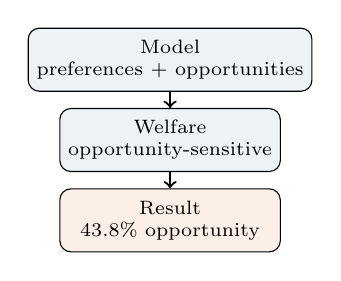
\begin{tikzpicture}[
  box/.style={draw,rounded corners,fill=cblue!8,minimum width=2.8cm,
    minimum height=0.8cm,font=\scriptsize,align=center,inner sep=3pt},
  scale=0.85]
  \node[box] (m) at (0,2.4) {Model\\preferences + opportunities};
  \node[box] (w) at (0,1.2) {Welfare\\opportunity-sensitive};
  \node[box,fill=corange!12] (r) at (0,0) {Result\\43.8\% opportunity};
  \draw[->,thick] (m) -- (w);
  \draw[->,thick] (w) -- (r);
\end{tikzpicture}
\end{column}
\end{columns}
\end{frame}

% ---- SLIDE 3: Why economists should care ----------------------------
\begin{frame}{Outcomes do not reveal the same thing for everyone}

\begin{itemize}
\item The same observed bundle can be a \textbf{chosen optimum} for one person and a \textbf{constrained second-best} for another
\item If opportunities are omitted, standard models absorb them into \textbf{tastes}
\item That distorts both the \textbf{positive} interpretation (preference heterogeneity) and the \textbf{normative} interpretation (who is truly worse off)
\item This matters for how economists think about \textbf{compensation}, \textbf{responsibility}, and \textbf{redistribution}
\end{itemize}

\vfill
\begin{center}
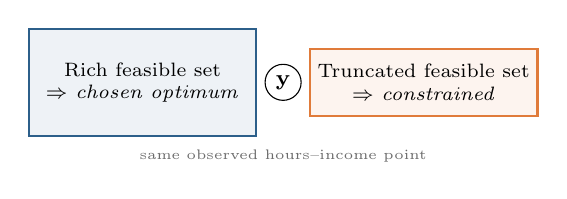
\begin{tikzpicture}[scale=0.85]
  \draw[thick,cblue,fill=cblue!8] (-3.8,-0.8) rectangle (-0.4,0.8);
  \draw[thick,corange,fill=corange!8] (0.4,-0.5) rectangle (3.8,0.5);
  \node[align=center,font=\scriptsize] at (-2.1,0) {Rich feasible set\\$\Rightarrow$ \emph{chosen optimum}};
  \node[align=center,font=\scriptsize] at (2.1,0)  {Truncated feasible set\\$\Rightarrow$ \emph{constrained}};
  \node[font=\footnotesize,fill=white,draw,circle,inner sep=2pt] at (0,0) {\textbf{y}};
  \node[font=\tiny,cgrey] at (0,-1.1) {same observed hours--income point};
\end{tikzpicture}
\end{center}
\end{frame}

\section{Literature}

% ---- SLIDE 4: Literature positioning --------------------------------
\begin{frame}{This paper sits at the intersection of four literatures}

\begin{center}
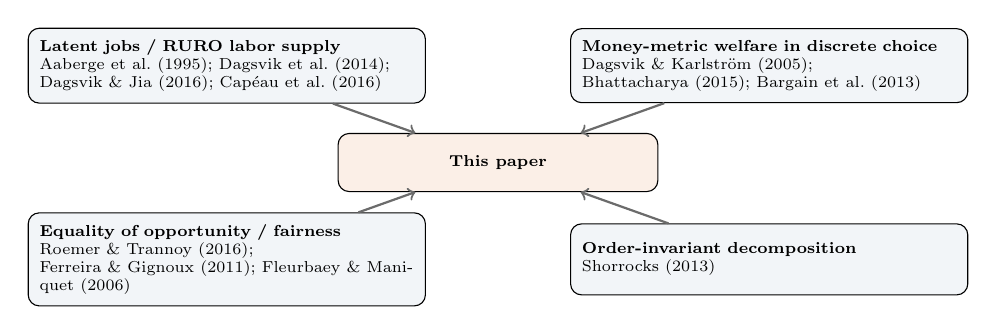
\begin{tikzpicture}[
  lit/.style={draw,rounded corners,fill=cblue!6,text width=5.8cm,
    minimum height=1.1cm,font=\scriptsize,align=left,inner sep=5pt},
  me/.style={draw,rounded corners,fill=corange!12,text width=4.6cm,
    minimum height=0.9cm,font=\scriptsize\bfseries,align=center,inner sep=5pt},
  scale=0.82, transform shape]
  \node[lit] (a) at (-4.2, 1.5) {%
    \textbf{Latent jobs / RURO labor supply}\\
    Aaberge et al.\ (1995); Dagsvik et al.\ (2014);\\
    Dagsvik \& Jia (2016); Cap\'eau et al.\ (2016)};
  \node[lit] (b) at (4.2, 1.5) {%
    \textbf{Money-metric welfare in discrete choice}\\
    Dagsvik \& Karlstr\"om (2005);\\
    Bhattacharya (2015); Bargain et al.\ (2013)};
  \node[lit] (c) at (-4.2,-1.5) {%
    \textbf{Equality of opportunity / fairness}\\
    Roemer \& Trannoy (2016);\\
    Ferreira \& Gignoux (2011); Fleurbaey \& Maniquet (2006)};
  \node[lit] (d) at (4.2,-1.5) {%
    \textbf{Order-invariant decomposition}\\
    Shorrocks (2013)};
  \node[me] (e) at (0,0) {This paper};
  \draw[->,thick,cgrey] (a) -- (e);
  \draw[->,thick,cgrey] (b) -- (e);
  \draw[->,thick,cgrey] (c) -- (e);
  \draw[->,thick,cgrey] (d) -- (e);
\end{tikzpicture}
\end{center}

\vspace{-0.2cm}
\scriptsize\textcolor{cgrey}{The unusual feature is not structural labor supply alone, but treating the estimated opportunity mechanism as a first-class distributive primitive.}
\end{frame}

% ---- SLIDE 5: What they do / what I do ------------------------------
\begin{frame}{Existing papers stop too early; I connect behavior, welfare, and fairness}

\footnotesize
\begin{tabular}{@{}>{\raggedright\arraybackslash}p{5.2cm} >{\raggedright\arraybackslash}p{5.2cm}@{}}
\toprule
\textbf{What they do} & \textbf{What I do} \\
\midrule
Constrained labor-supply papers stop at \textbf{fit, elasticities, or reform simulation}
& Estimate \textbf{opportunities}, translate them into \textbf{welfare}, and \textbf{decompose welfare inequality} \\[6pt]
Welfare papers with heterogeneous preferences stop before \textbf{explicit opportunity modeling}
& Construct welfare \textbf{conditional on the estimated feasible set}, not on a universal menu \\[6pt]
Equality-of-opportunity papers use \textbf{reduced-form circumstance partitions}
& Use \textbf{structurally estimated job-opportunity distributions} as the circumstance object \\[6pt]
Decomposition methods require \textbf{analyst-defined counterfactuals}
& Define counterfactuals from the \textbf{estimated preference and opportunity blocks} \\
\bottomrule
\end{tabular}

\vfill
\scriptsize\textcolor{cgrey}{The contribution is integration: a latent-jobs labor-supply model, an opportunity-sensitive welfare metric, and a structural decomposition of welfare inequality in one design.}
\end{frame}

\section{Design \& Result}

% ---- SLIDE 6: Belgium baseline --------------------------------------
\begin{frame}{Belgium is the clean first application}

\begin{columns}[T]
\begin{column}{0.52\textwidth}
\begin{itemize}
\item Data: \textbf{Belgian EU-SILC} + EUROMOD baseline tax-benefit rules
\item Sample: \emphnum{3,284} childless single women aged \emphnum{25--54}
\item 16 job packages: non-employment + 5 hours bins $\times$ 3 wage terciles
\item Opportunity heterogeneity: region~$\times$~education
\item Preference heterogeneity: age, age$^2$, two latent taste types
\end{itemize}

\medskip
\scriptsize\textcolor{cgrey}{Design strips out joint household choice, childcare, and self-employment --- keeping the first paper focused on the opportunity-vs-preference question.}
\end{column}
\begin{column}{0.44\textwidth}
\centering
\footnotesize
\begin{tabular}{@{}l r@{}}
\toprule
\textbf{Statistic} & \textbf{Value} \\
\midrule
Employment rate        & 77.6\% \\
Mean weekly hours      & 34.9   \\
Mean hourly wage       & \texteuro15.8 \\
Mean disp.\ income     & \texteuro1,694 \\
\midrule
Flanders               & 56.8\% \\
Wallonia                & 30.9\% \\
Brussels                & 12.3\% \\
\midrule
Low education           & 25.9\% \\
Medium education        & 42.5\% \\
High education          & 31.6\% \\
\bottomrule
\end{tabular}
\end{column}
\end{columns}
\end{frame}

% ---- SLIDE 7: Main result ------------------------------------------
\begin{frame}{Unequal opportunities explain a large share of welfare inequality}

\begin{columns}[T]
\begin{column}{0.48\textwidth}
\vspace{-0.1cm}
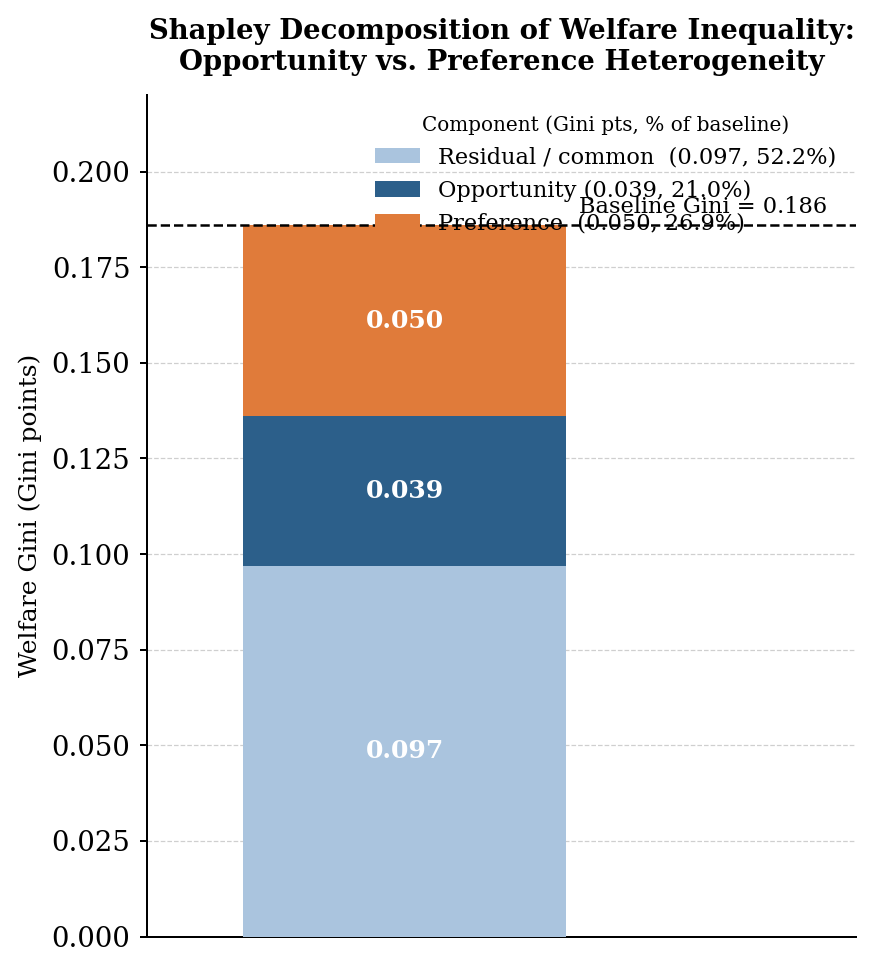
\includegraphics[width=\linewidth]{figures/figure_decomposition_shares.png}
\end{column}
\begin{column}{0.50\textwidth}
\footnotesize
\begin{tabular}{@{}l r@{}}
\toprule
\textbf{Scenario} & \textbf{Welfare Gini} \\
\midrule
Baseline              & \emphnum{0.186} \\
Opp.\ equalized       & 0.151 \\
Pref.\ equalized      & 0.140 \\
Both equalized        & 0.097 \\
\bottomrule
\end{tabular}

\medskip
\begin{tabular}{@{}l r r@{}}
\toprule
\textbf{Component} & \textbf{Gini pts} & \textbf{\% expl.} \\
\midrule
Opportunity   & \emphnum{0.039} & \emphnum{43.8\%} \\
Preference    & \emphpref{0.050} & 56.2\% \\
\bottomrule
\end{tabular}

\medskip
\scriptsize
Opportunities: \emphnum{21.0\%} of baseline welfare Gini\\
Income Gini 0.164 vs welfare Gini \emphnum{0.186}
\end{column}
\end{columns}
\end{frame}

% ====================================================================
%  CONTINUATION — SLIDES 8–22  (full talk)
% ====================================================================

\section{Data \& Model}

% ---- SLIDE 8: Raw data motivation ----------------------------------
\begin{frame}{The raw data already show structured opportunity differences}

\begin{columns}[T]
\begin{column}{0.48\textwidth}
\footnotesize
\textbf{Employment rate by region $\times$ education}\\[4pt]
\begin{tabular}{@{}l ccc@{}}
\toprule
 & Flan. & Wall. & Bxl. \\
\midrule
Low ed.    & 72.4\% & 64.0\% & \cellcolor{corange!15}\emphnum{62.4\%} \\
Medium ed. & 79.3\% & 73.6\% & 71.2\% \\
High ed.   & \cellcolor{cblue!10}\emphnum{86.5\%} & 83.8\% & 82.4\% \\
\bottomrule
\end{tabular}

\bigskip
\begin{itemize}\footnotesize
\item Employment ranges from \emphnum{62.4\%} to \emphnum{86.5\%}
\item Non-employment: \emphnum{22.4\%} of the sample
\item Standard-hours work is the dominant mode
\end{itemize}
\end{column}
\begin{column}{0.48\textwidth}
\centering
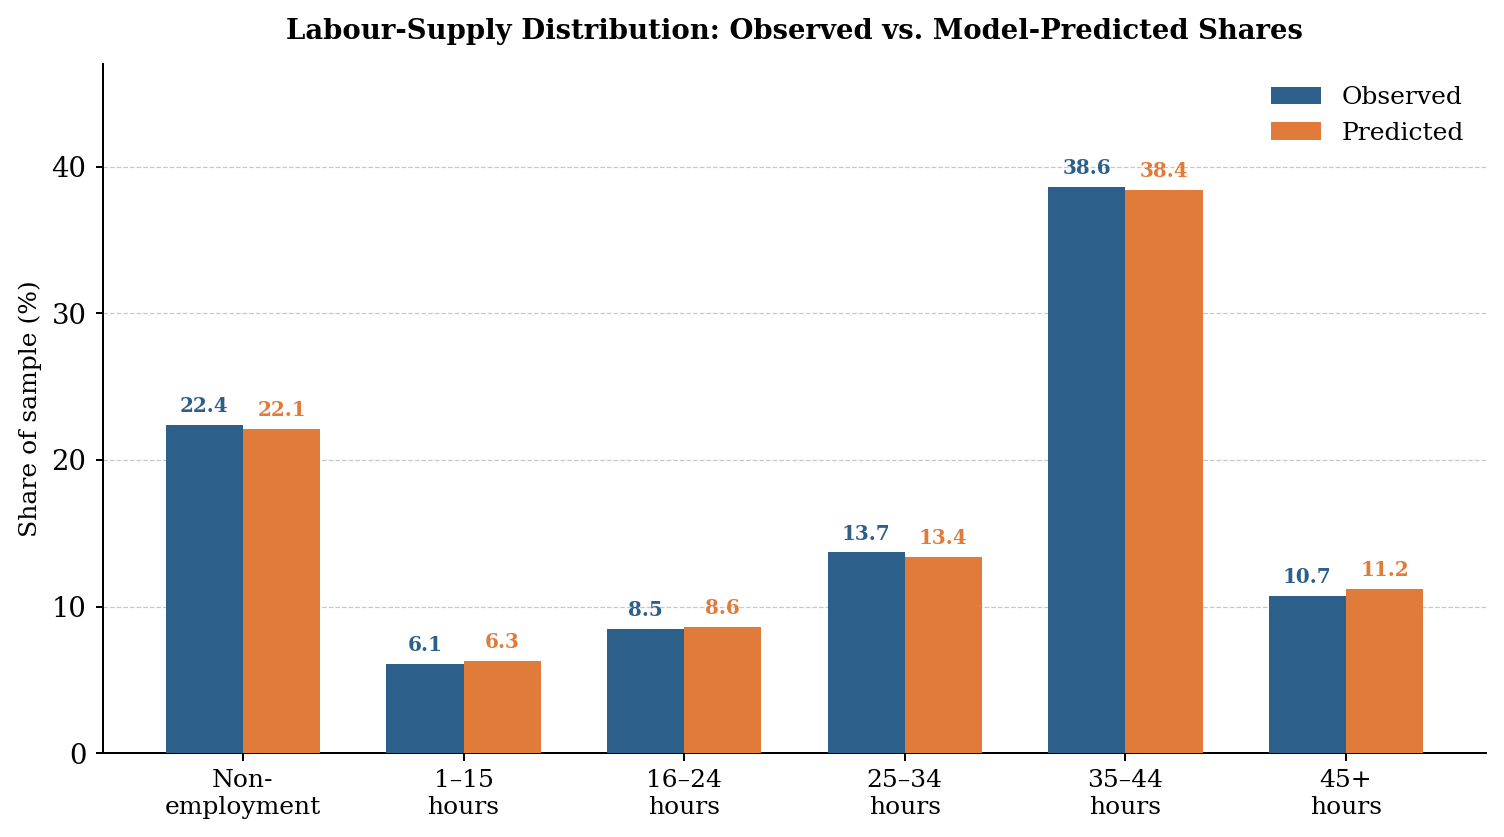
\includegraphics[width=\linewidth]{figures/figure_fit.png}
\end{column}
\end{columns}

\vfill
\scriptsize\textcolor{cgrey}{A credible model must fit these region $\times$ education gradients, not just overall participation.}
\end{frame}

% ---- SLIDE 9: 16 job packages --------------------------------------
\begin{frame}{The 16 job packages make latent opportunities operational}

\begin{columns}[T]
\begin{column}{0.55\textwidth}
\begin{itemize}
\item Alternatives: non-employment + 5 hours bins $\times$ 3 wage terciles
\item Hours bins: 1--15,\; 16--24,\; 25--34,\; 35--44,\; 45+
\item The \textbf{preference block} ranks accessible packages
\item The \textbf{opportunity block} governs access
\end{itemize}

\medskip
\scriptsize\textcolor{cgrey}{Equalizing opportunities means equalizing access to a defined distribution of wage--hours packages, not shifting an abstract parameter.}
\end{column}
\begin{column}{0.42\textwidth}
\centering
\footnotesize
\begin{tabular}{@{}c|ccc@{}}
\toprule
 & Low w. & Mid w. & High w. \\
\midrule
1--15\,h   & \cellcolor{cblue!6}  & \cellcolor{cblue!6}  & \cellcolor{cblue!6}  \\
16--24\,h  & \cellcolor{cblue!8}  & \cellcolor{cblue!8}  & \cellcolor{cblue!8}  \\
25--34\,h  & \cellcolor{cblue!12} & \cellcolor{cblue!12} & \cellcolor{cblue!12} \\
35--44\,h  & \cellcolor{cblue!18} & \cellcolor{cblue!18} & \cellcolor{cblue!18} \\
45$+$\,h   & \cellcolor{cblue!8}  & \cellcolor{cblue!8}  & \cellcolor{cblue!8}  \\
\bottomrule
\end{tabular}
\\[4pt]
\scriptsize $+$\; non-employment\\[6pt]

\begin{tikzpicture}[scale=0.7]
  \draw[thick,cblue,->] (0,1.2) -- (0,0) node[midway,left,font=\scriptsize] {Pref.};
  \draw[thick,corange,->] (1.2,1.2) -- (1.2,0) node[midway,right,font=\scriptsize] {Opp.};
\end{tikzpicture}
\end{column}
\end{columns}
\end{frame}

% ---- SLIDE 10: Identification --------------------------------------
\begin{frame}{Identification is simple to state: ranking versus access}

\begin{itemize}
\item The identification challenge is to separate \textbf{how people rank packages} from \textbf{which packages are available}
\item Region $\times$ education disciplines the opportunity block
\item Age and latent taste types discipline the preference block
\item Welfare is then computed \textbf{conditional on the feasible set}, not on a universal menu
\end{itemize}

\vfill
\begin{center}
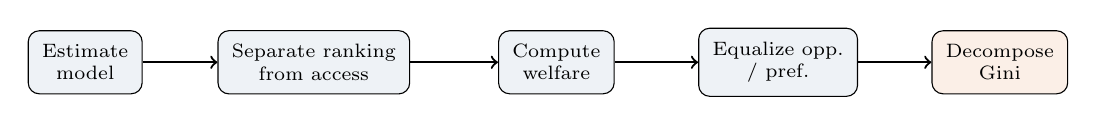
\begin{tikzpicture}[
  box/.style={draw,rounded corners,fill=cblue!8,minimum height=0.7cm,
    font=\scriptsize,align=center,inner sep=5pt},
  scale=0.88]
  \node[box] (a) at (0,0) {Estimate\\model};
  \node[box] (b) at (3.3,0) {Separate ranking\\from access};
  \node[box] (c) at (6.8,0) {Compute\\welfare};
  \node[box] (d) at (10,0) {Equalize opp.\\ / pref.};
  \node[box,fill=corange!12] (e) at (13.2,0) {Decompose\\Gini};
  \draw[->,thick] (a) -- (b);
  \draw[->,thick] (b) -- (c);
  \draw[->,thick] (c) -- (d);
  \draw[->,thick] (d) -- (e);
\end{tikzpicture}
\end{center}
\end{frame}

\section{Estimation}

% ---- SLIDE 11: Preference estimates ---------------------------------
\begin{frame}{Preference heterogeneity is meaningful, but not a catch-all residual}

\begin{columns}[T]
\begin{column}{0.52\textwidth}
\footnotesize
\begin{tabular}{@{}l r r@{}}
\toprule
\textbf{Parameter} & \textbf{Est.} & \textbf{SE} \\
\midrule
Log disp.\ income              & 2.946*** & 0.188 \\
Log leisure, Type~1            & 1.428*** & 0.116 \\
Type~2 shift                   & 0.612*** & 0.141 \\
Age/10 $\times$ log leisure    & 0.084*** & 0.029 \\
(Age/10)$^2$ $\times$ log leisure & $-$0.010*** & 0.003 \\
Work fixed cost                & $-$1.324*** & 0.182 \\
Type~2 logit intercept         & $-$0.447*** & 0.118 \\
Type~2 pop.\ share             & 0.390*** & 0.028 \\
\bottomrule
\multicolumn{3}{@{}l@{}}{\scriptsize *** $p<0.01$,\; ** $p<0.05$,\; * $p<0.10$}
\end{tabular}
\end{column}
\begin{column}{0.44\textwidth}
\begin{itemize}\footnotesize
\item Income enters positively; leisure matters strongly
\item Two latent types: leisure coeff.\ \emphpref{1.43} (T1); \emphpref{2.04} (T2)
\item Type~2 share: \emphpref{39\%}
\item Work fixed cost is sizable ($-$1.324)
\item Marginal value of leisure rises with age, concavely
\end{itemize}

\medskip
\scriptsize
\textcolor{cgrey}{Preferences do not vanish once opportunities are modeled. In the decomposition, preferences still explain slightly more than opportunities.}
\end{column}
\end{columns}
\end{frame}

% ---- SLIDE 12: Opportunity estimates --------------------------------
\begin{frame}{The opportunity estimates reveal a real labor-market structure}

\begin{columns}[T]
\begin{column}{0.52\textwidth}
\footnotesize
\textbf{Log total offer intensity ($\ln q_i$)}\\[4pt]
\begin{tabular}{@{}l r r@{}}
\toprule
\textbf{Parameter} & \textbf{Est.} & \textbf{SE} \\
\midrule
Wallonia                   & $-$0.150** & 0.061 \\
Brussels                   & $-$0.192*** & 0.071 \\
Low education              & $-$0.108** & 0.051 \\
High education             & 0.151** & 0.062 \\
Wallonia $\times$ Low ed.  & $-$0.109* & 0.060 \\
Brussels $\times$ Low ed.  & $-$0.126* & 0.071 \\
\bottomrule
\end{tabular}

\bigskip
\textbf{Implied relative offer intensity}\\
\scriptsize Ref: Flanders / Medium = 1.00\\[4pt]
\footnotesize
\begin{tabular}{@{}l ccc@{}}
\toprule
 & Flan. & Wall. & Bxl. \\
\midrule
Low    & 0.90 & 0.69 & \emphnum{0.65} \\
Medium & 1.00 & 0.86 & 0.83 \\
High   & \emphnum{1.16} & 1.01 & 0.99 \\
\bottomrule
\end{tabular}
\end{column}
\begin{column}{0.44\textwidth}
\begin{itemize}\footnotesize
\item Total offer intensity lowest for low-educated women outside Flanders
\item Range: \emphnum{0.65} to \emphnum{1.16}
\item Standard-hours packages much more prevalent than fringe-hours jobs
\item Top-wage packages relatively scarcer
\end{itemize}

\medskip
\scriptsize
\textcolor{cgrey}{The opportunity block is not a nuisance term; it is an estimated, economically interpretable map of unequal access to work.}
\end{column}
\end{columns}
\end{frame}

% ---- SLIDE 13: Benchmark fit ----------------------------------------
\begin{frame}{The benchmark misses exactly the gradients the opportunity block explains}

\begin{columns}[T]
\begin{column}{0.48\textwidth}
\scriptsize
\textbf{Model comparison}\\[2pt]
\begin{tabular}{@{}l cc@{}}
\toprule
 & \textbf{Full} & \textbf{Bench.} \\
\midrule
Pseudo-$R^2$    & \emphnum{0.271} & 0.214 \\
Exact hit rate   & \emphnum{39.2\%} & 33.8\% \\
Empl.\ classif. & 82.4\% & --- \\
\bottomrule
\end{tabular}

\medskip
\textbf{Employment rate: observed vs predicted}\\[2pt]
\begin{tabular}{@{}l cc@{}}
\toprule
\textbf{Cell} & \textbf{Obs.} & \textbf{Pred.} \\
\midrule
Flan./Low   & 72.4 & 73.0 \\
Flan./Med   & 79.3 & 78.9 \\
Flan./High  & 86.5 & 85.9 \\
Wall./Low   & 64.0 & 64.8 \\
Wall./Med   & 73.6 & 74.0 \\
Wall./High  & 83.8 & 83.0 \\
Bxl./Low    & 62.4 & 63.5 \\
Bxl./Med    & 71.2 & 72.0 \\
Bxl./High   & 82.4 & 81.7 \\
\bottomrule
\end{tabular}
\end{column}
\begin{column}{0.48\textwidth}
\begin{itemize}\footnotesize
\item Full model improves pseudo-$R^2$ from 0.214 to \emphnum{0.271}
\item Exact hit rate: 33.8\% $\rightarrow$ \emphnum{39.2\%}
\item Main gain: recovering \textbf{region $\times$ education gradients} the benchmark compresses
\item If the benchmark flattens those gradients, it absorbs them into \textbf{preferences}
\end{itemize}

\medskip
\scriptsize
\textcolor{cgrey}{Explicit opportunities improve fit precisely where the omitted-opportunity problem should matter most.}
\end{column}
\end{columns}
\end{frame}

% ---- SLIDE 14: Elasticities ----------------------------------------
\begin{frame}{Elasticities validate the structure, but do not drive the contribution}

\begin{columns}[T]
\begin{column}{0.52\textwidth}
\centering
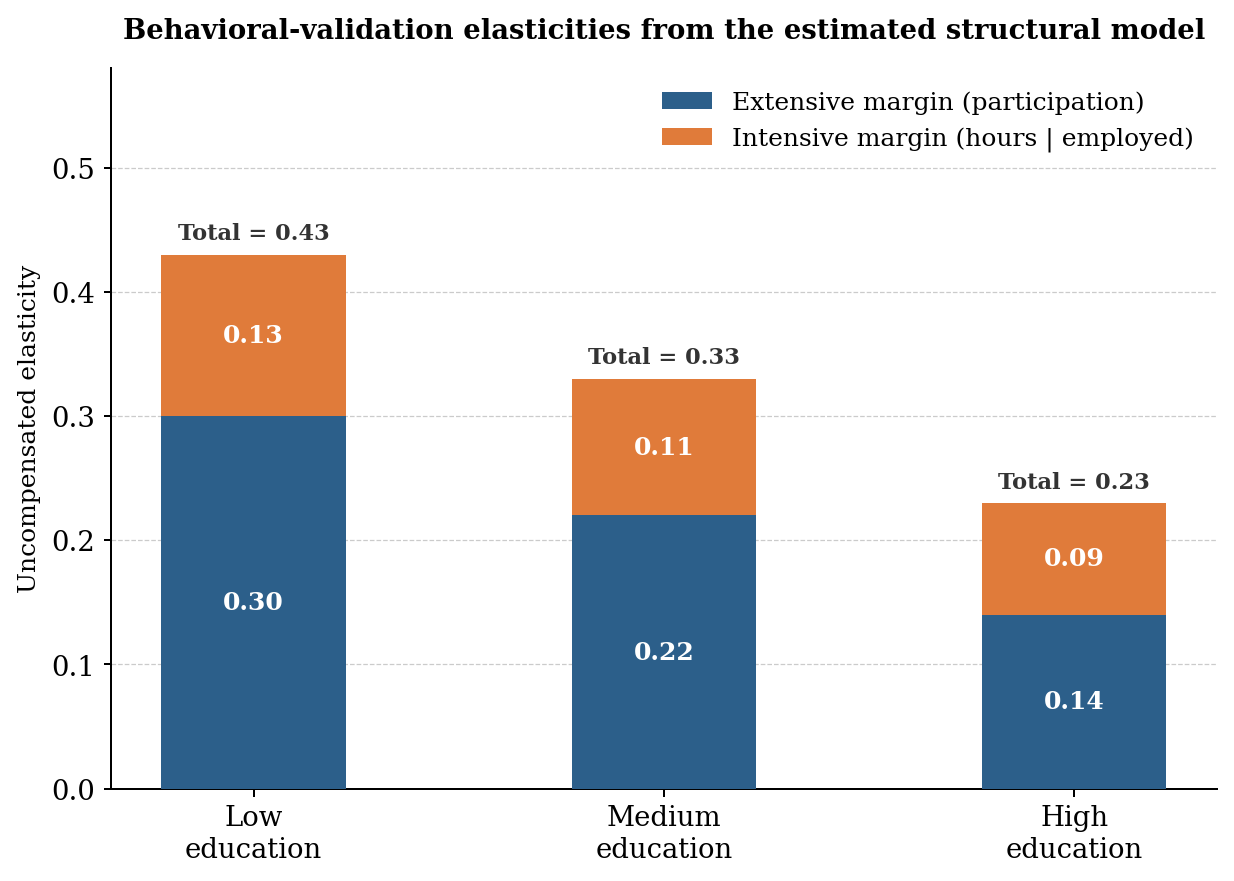
\includegraphics[width=\linewidth]{figures/figure_elasticities.png}
\end{column}
\begin{column}{0.44\textwidth}
\footnotesize
Uncompensated arc elasticities from a 1\% proportional wage increase, holding job-offer probabilities fixed

\bigskip
\begin{tabular}{@{}l ccc@{}}
\toprule
 & \textbf{Ext.} & \textbf{Int.} & \textbf{Total} \\
\midrule
Overall & 0.21 & 0.11 & \emphnum{0.32} \\
Low ed. & 0.30 & 0.13 & \emphnum{0.43} \\
Med.\ ed. & 0.22 & 0.11 & 0.33 \\
High ed. & 0.14 & 0.09 & 0.23 \\
\bottomrule
\end{tabular}

\bigskip
\scriptsize
\textcolor{cgrey}{This is a behavioral-validation result. The paper's contribution remains the welfare measure and its decomposition.}
\end{column}
\end{columns}
\end{frame}

\section{Decomposition}

% ---- SLIDE 15: Welfare ≠ income inequality --------------------------
\begin{frame}{Welfare inequality is not the same object as income inequality}

\begin{columns}[T]
\begin{column}{0.48\textwidth}
\footnotesize
\begin{tabular}{@{}l r@{}}
\toprule
\textbf{Welfare distribution} & \textbf{Value} \\
\midrule
Mean monthly welfare          & \texteuro1,718 \\
Median monthly welfare        & \texteuro1,681 \\
10th percentile               & \texteuro1,079 \\
90th percentile               & \texteuro2,452 \\
\bottomrule
\end{tabular}

\bigskip
\begin{itemize}\footnotesize
\item Two individuals with similar income can have different welfare once one reaches that outcome from a much poorer feasible set
\item Welfare inequality \textbf{rises} when we evaluate people not only by what they earn, but by what they can access
\end{itemize}
\end{column}
\begin{column}{0.48\textwidth}
\centering
\vspace{0.5cm}
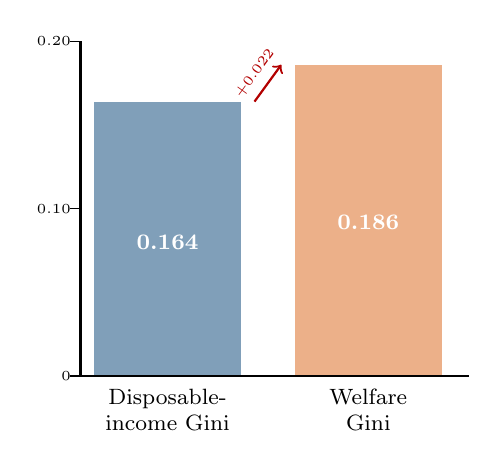
\begin{tikzpicture}[scale=0.85]
  % bars
  \fill[cblue!60] (0,0) rectangle (2.2,4.1);
  \fill[corange!60] (3.0,0) rectangle (5.2,4.65);
  % labels
  \node[font=\footnotesize,align=center] at (1.1,-0.5) {Disposable-\\income Gini};
  \node[font=\footnotesize,align=center] at (4.1,-0.5) {Welfare\\Gini};
  \node[font=\bfseries\footnotesize,white] at (1.1,2.0) {0.164};
  \node[font=\bfseries\footnotesize,white] at (4.1,2.3) {0.186};
  % axis
  \draw[thick] (-0.2,0) -- (5.6,0);
  \draw[thick] (-0.2,0) -- (-0.2,5.0);
  \foreach \y/\lab in {0/0,2.5/0.10,5.0/0.20}
    {\draw (-0.35,\y) -- (-0.2,\y) node[left,font=\tiny] {\lab};}
  % arrow
  \draw[->,thick,red!70!black] (2.4,4.1) -- (2.8,4.65)
    node[midway,above,font=\tiny,sloped] {+0.022};
\end{tikzpicture}
\end{column}
\end{columns}
\end{frame}

% ---- SLIDE 16: Transparent counterfactuals --------------------------
\begin{frame}{The decomposition is built from transparent counterfactuals}

\begin{center}
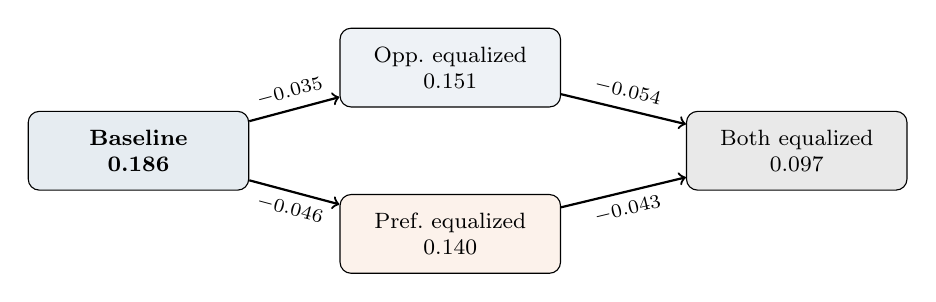
\begin{tikzpicture}[
  box/.style={draw,rounded corners,minimum width=2.8cm,minimum height=1.0cm,
    font=\footnotesize,align=center,inner sep=4pt},
  scale=0.88]
  \node[box,fill=cblue!12,font=\footnotesize\bfseries] (bl) at (0,0) {Baseline\\0.186};
  \node[box,fill=cblue!8] (oe) at (4.5,1.2) {Opp.\ equalized\\0.151};
  \node[box,fill=corange!10] (pe) at (4.5,-1.2) {Pref.\ equalized\\0.140};
  \node[box,fill=cgrey!15] (be) at (9.5,0) {Both equalized\\0.097};
  \draw[->,thick] (bl) -- (oe) node[midway,above,font=\scriptsize,sloped] {$-$0.035};
  \draw[->,thick] (bl) -- (pe) node[midway,below,font=\scriptsize,sloped] {$-$0.046};
  \draw[->,thick] (oe) -- (be) node[midway,above,font=\scriptsize,sloped] {$-$0.054};
  \draw[->,thick] (pe) -- (be) node[midway,below,font=\scriptsize,sloped] {$-$0.043};
\end{tikzpicture}
\end{center}

\bigskip
\begin{itemize}
\item Each counterfactual welfare Gini comes from an explicit equalization exercise
\item The attribution uses an \textbf{order-invariant Shapley--Shorrocks} rule
\item No dependence on the sequence in which factors are removed
\end{itemize}

\vfill
\scriptsize\textcolor{cgrey}{The decomposition rests on explicit structural equalization exercises, not on a black-box regression residual.}
\end{frame}

% ---- SLIDE 17: Main decomposition result ----------------------------
\begin{frame}{The main decomposition result is balanced, not rhetorical}

\begin{columns}[T]
\begin{column}{0.48\textwidth}
\centering
\vspace{0.2cm}
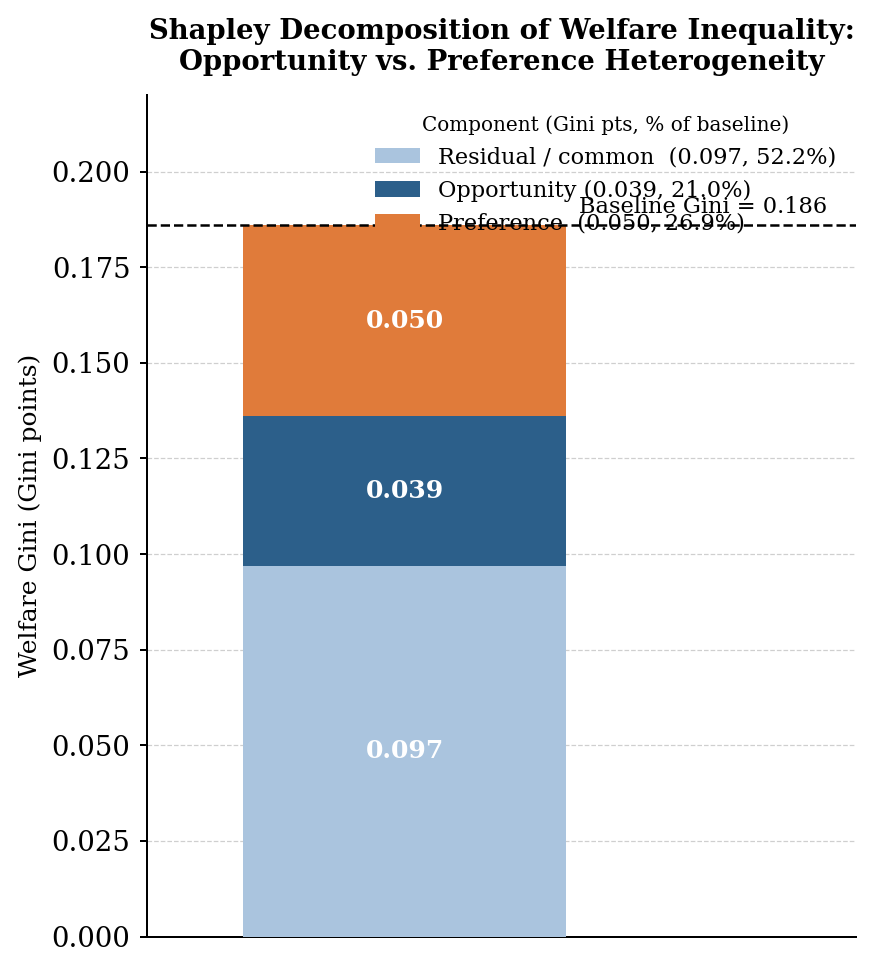
\includegraphics[width=\linewidth]{figures/figure_decomposition_shares.png}
\end{column}
\begin{column}{0.48\textwidth}
\footnotesize
\begin{tabular}{@{}l r r@{}}
\toprule
\textbf{Component} & \textbf{Gini pts} & \textbf{\% explained} \\
\midrule
\textcolor{cblue}{Opportunity}  & \emphnum{0.039} & \emphnum{43.8\%} \\
\textcolor{corange}{Preference} & \emphpref{0.050} & \emphpref{56.2\%} \\
Residual/common                 & 0.097 & --- \\
\midrule
Baseline Gini                   & 0.186 & \\
\bottomrule
\end{tabular}

\bigskip
\begin{itemize}\footnotesize
\item Opportunities: \emphnum{21.0\%} of baseline welfare Gini
\item Preferences: \emphpref{26.9\%} of baseline welfare Gini
\item The result is strongest \emph{because} it is balanced
\item Opportunities matter a great deal, but the paper does not claim they explain everything
\end{itemize}
\end{column}
\end{columns}
\end{frame}

% ---- SLIDE 18: Responsibility sensitivity ---------------------------
\begin{frame}{The opportunity contribution is criterion-dependent, but does not disappear}

\begin{columns}[T]
\begin{column}{0.52\textwidth}
\centering
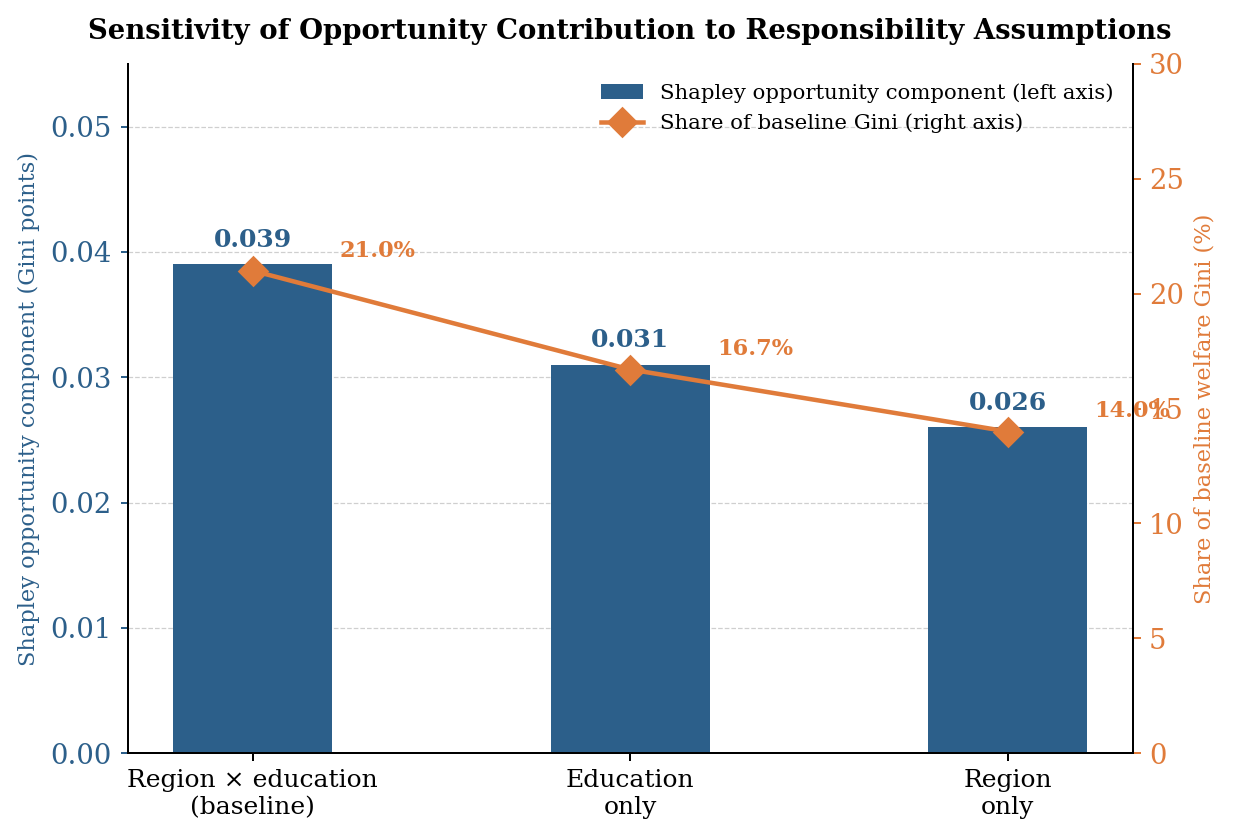
\includegraphics[width=\linewidth]{figures/figure_responsibility_sensitivity.png}
\end{column}
\begin{column}{0.44\textwidth}
\footnotesize
\begin{tabular}{@{}l cc@{}}
\toprule
\textbf{Compensable}              & \textbf{Opp.} & \textbf{\% of} \\
\textbf{definition}               & \textbf{comp.} & \textbf{Gini} \\
\midrule
Region $\times$ ed.\ (baseline) & \emphnum{0.039} & \emphnum{21.0\%} \\
Education only                    & 0.031 & 16.7\% \\
Region only                       & 0.026 & 14.0\% \\
\bottomrule
\end{tabular}

\bigskip
\begin{itemize}\footnotesize
\item The opportunity contribution is \textbf{criterion-dependent}
\item It declines as the responsibility stance tightens
\item But it does not vanish: \emphnum{14--21\%} of baseline Gini
\item The contribution is the \textbf{decomposition itself}, not one preferred fairness metric
\end{itemize}
\end{column}
\end{columns}
\end{frame}

\section{Conclusion}

% ---- SLIDE 19: Why decomposition > welfare levels -------------------
\begin{frame}{Decomposition matters more than welfare levels alone}

\begin{columns}[T]
\begin{column}{0.48\textwidth}
\begin{itemize}
\item A welfare level tells us \textbf{where} people stand
\item A decomposition tells us \textbf{why} inequality exists
\item Policy implications differ if inequality is driven by \textbf{job access} rather than \textbf{preferences}
\item That is why the paper's main object is a \textbf{decomposition}, not a ranking
\end{itemize}
\end{column}
\begin{column}{0.48\textwidth}
\centering
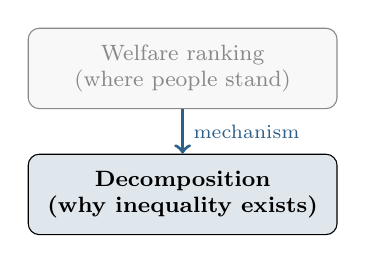
\begin{tikzpicture}[scale=0.8]
  % faded ranking
  \node[draw,rounded corners,fill=cgrey!10,text width=3.5cm,align=center,
    font=\footnotesize,inner sep=6pt,opacity=0.45] (rank) at (0,2)
    {Welfare ranking\\(where people stand)};
  % emphasized decomposition
  \node[draw,rounded corners,fill=cblue!15,text width=3.5cm,align=center,
    font=\footnotesize\bfseries,inner sep=6pt] (dec) at (0,0)
    {Decomposition\\(why inequality exists)};
  \draw[->,very thick,cblue] (rank) -- (dec)
    node[midway,right,font=\scriptsize] {mechanism};
\end{tikzpicture}
\end{column}
\end{columns}

\vfill
\scriptsize\textcolor{cgrey}{Papers like Bargain et al.\ (2013) show welfare rankings are sensitive to preferences and metric choice. This paper delivers a mechanism question instead.}
\end{frame}

% ---- SLIDE 20: Belgium vs Europe ------------------------------------
\begin{frame}{The Belgium baseline is a paper; Europe is an agenda}

\begin{columns}[T]
\begin{column}{0.48\textwidth}
\centering
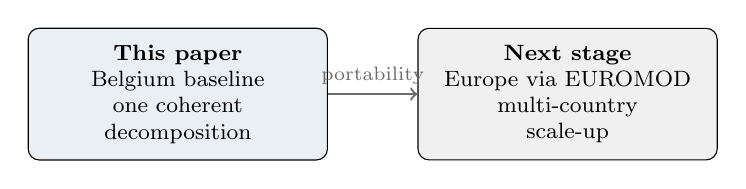
\begin{tikzpicture}[
  box/.style={draw,rounded corners,minimum width=3.8cm,minimum height=1.5cm,
    font=\footnotesize,align=center,inner sep=6pt},
  scale=0.9]
  \node[box,fill=cblue!10] (be) at (0,0) {\textbf{This paper}\\Belgium baseline\\one coherent\\decomposition};
  \node[box,fill=cgrey!10] (eu) at (5.5,0) {\textbf{Next stage}\\Europe via EUROMOD\\multi-country\\scale-up};
  \draw[->,thick,cgrey] (be) -- (eu)
    node[midway,above,font=\scriptsize] {portability};
\end{tikzpicture}
\end{column}
\begin{column}{0.48\textwidth}
\begin{itemize}\footnotesize
\item Belgium provides the clean \textbf{first proof of concept}
\item EUROMOD portability makes multi-country extension \textbf{feasible}
\item Scaling too early risks a \textbf{ranking exercise}
\item Europe belongs in the broader agenda, not in the paper's identity
\end{itemize}
\end{column}
\end{columns}
\end{frame}

% ---- SLIDE 21: Narrow by design ------------------------------------
\begin{frame}{The paper is narrow by design, not narrow by ambition}

\footnotesize
\begin{tabular}{@{}p{4.5cm} p{6.2cm}@{}}
\toprule
\textbf{What I narrow} & \textbf{Why that strengthens the paper} \\
\midrule
Opportunity block is parsimonious (region $\times$ education)
& Keeps identification transparent; avoids over-fitting \\[4pt]
Sample is clean (childless single women)
& Removes joint household choice, childcare, self-employment \\[4pt]
Decomposition uses two factors only
& Shapley attribution is exact and interpretable \\[4pt]
One country baseline
& Establishes the mechanism before scaling up \\
\bottomrule
\end{tabular}

\bigskip
\begin{center}
\textbf{Strategy:}\; interpretability first, scale-up second
\end{center}
\end{frame}

% ---- SLIDE 22: Closing ----------------------------------------------
\begin{frame}{What the committee should remember}

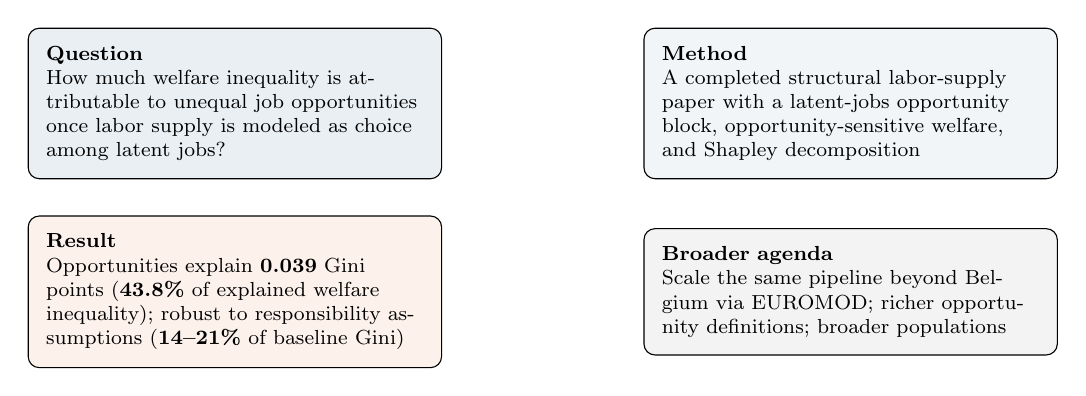
\begin{tikzpicture}[
  every node/.style={draw,rounded corners,align=left,inner sep=7pt,
    font=\footnotesize, text width=0.43\textwidth},
  scale=0.92, transform shape]
  \node[fill=cblue!10] (q) at (0,0) {%
    \textbf{Question}\\
    How much welfare inequality is attributable to unequal job opportunities once labor supply is modeled as choice among latent jobs?};
  \node[fill=cblue!6] (m) at (8.5,0) {%
    \textbf{Method}\\
    A completed structural labor-supply paper with a latent-jobs opportunity block, opportunity-sensitive welfare, and Shapley decomposition};
  \node[fill=corange!10] (r) at (0,-2.6) {%
    \textbf{Result}\\
    Opportunities explain \textbf{0.039} Gini points (\textbf{43.8\%} of explained welfare inequality); robust to responsibility assumptions (\textbf{14--21\%} of baseline Gini)};
  \node[fill=cgrey!8] (a) at (8.5,-2.6) {%
    \textbf{Broader agenda}\\
    Scale the same pipeline beyond Belgium via EUROMOD; richer opportunity definitions; broader populations};
\end{tikzpicture}
\end{frame}


% ====================================================================
%  APPENDIX / BACKUP SLIDES
% ====================================================================
\appendix

\begin{frame}[plain]
\vfill
\begin{center}
\Large\bfseries Appendix / Backup Slides
\end{center}
\vfill
\end{frame}

% ---- APPENDIX 1: Full literature map --------------------------------
\begin{frame}{Appendix 1: Full Named-Paper Literature Map}

\scriptsize
\begin{tabular}{@{}>{\bfseries\raggedright}p{2.8cm} p{8.5cm}@{}}
\toprule
\textbf{Strand} & \textbf{Named anchors} \\
\midrule
Latent jobs / RURO labor supply
& Aaberge, Colombino \& Str\o m (1995); Dagsvik, Jia \& Orsini (2014); Dagsvik \& Jia (2016); Cap\'eau, Decoster, De Sadeleer, Orsini, Pessl\'e \& Tojerow (2016) \\[4pt]
Money-metric welfare in discrete choice
& Dagsvik \& Karlstr\"om (2005); Bhattacharya (2015); Bargain, Decoster, Dolls, Neumann, Peichl \& Siegloch (2013) \\[4pt]
Equality of opportunity / fairness
& Roemer \& Trannoy (2016); Ferreira \& Gignoux (2011); Fleurbaey \& Maniquet (2006); Fleurbaey \& Schokkaert (2009) \\[4pt]
Order-invariant decomposition
& Shorrocks (2013); Audoly, Fortin \& Lemieux (2025) \\
\bottomrule
\end{tabular}

\bigskip
\centering
\scriptsize\textcolor{cgrey}{The paper's location: estimate latent opportunities $\rightarrow$ compute opportunity-sensitive welfare $\rightarrow$ Shapley--Shorrocks decompose welfare inequality + responsibility sensitivity.}
\end{frame}

% ---- APPENDIX 2: What they do / what I do (expanded) ----------------
\begin{frame}{Appendix 2: What They Do / What I Do (Expanded)}

\scriptsize
\begin{tabular}{@{}>{\raggedright}p{2.2cm} >{\raggedright}p{4.0cm} >{\raggedright\arraybackslash}p{4.8cm}@{}}
\toprule
\textbf{Strand} & \textbf{What they do} & \textbf{What I do} \\
\midrule
Constrained labor supply
& Estimate job-package models; use for fit, elasticities, reform simulations
& Use the same structure as \emph{input} into a welfare distribution; decompose welfare inequality via counterfactual opportunity equalization \\[4pt]
Money-metric welfare
& Develop/apply EV/CV welfare objects; welfare rankings across groups/countries
& Construct welfare \emph{conditional on heterogeneous feasible sets}, so constrained bundles are not misread as low-welfare choices \\[4pt]
Equality of opportunity
& Provide ethical language; measure between-type inequality with reduced-form partitions
& Operationalize opportunities as \emph{estimated job-opportunity distributions}; deliver responsibility-sensitive decomposition \\[4pt]
Decomposition
& Provide Shapley-value attributions once counterfactuals are defined
& Define counterfactuals in \emph{structural} terms and implement a two-factor Shapley--Shorrocks attribution of the welfare Gini \\
\bottomrule
\end{tabular}
\end{frame}

% ---- APPENDIX 3: Sample construction --------------------------------
\begin{frame}{Appendix 3: Sample Construction}

\centering
\footnotesize
\begin{tabular}{@{}l r@{}}
\toprule
\textbf{Step} & \textbf{Remaining} \\
\midrule
Belgian EU-SILC baseline population         & --- \\
Restrict to women aged 25--54               & --- \\
Drop partnered / married                    & --- \\
Drop women with dependent children          & --- \\
Drop self-employed                          & --- \\
Final estimation sample                     & 3,284 \\
\bottomrule
\end{tabular}

\bigskip
\begin{tabular}{@{}l r@{}}
\toprule
\textbf{Sample statistic} & \textbf{Value} \\
\midrule
Mean age                   & 39.7 \\
Employment rate            & 77.6\% \\
Mean weekly hours (empl.)  & 34.9 \\
Mean gross hourly wage     & \texteuro15.8 \\
Mean monthly disp.\ income & \texteuro1,694 \\
\bottomrule
\end{tabular}

\bigskip
\scriptsize\textcolor{cgrey}{Design restrictions remove avoidable sources of complexity while preserving sufficient heterogeneity for the opportunity block.}
\end{frame}

% ---- APPENDIX 4: Full structural estimates --------------------------
\begin{frame}{Appendix 4: Full Structural Estimates}

\begin{columns}[T]
\begin{column}{0.48\textwidth}
\centering
\footnotesize
\textbf{Preference block}\\[4pt]
\begin{tabular}{@{}l r r l@{}}
\toprule
\textbf{Parameter} & \textbf{Est.} & \textbf{SE} & \\
\midrule
Log disp.\ income         &  2.946 & (0.188) & *** \\
Log leisure, T1            &  1.428 & (0.116) & *** \\
T2 shift                   &  0.612 & (0.141) & *** \\
Age/10 $\times$ log leis.  &  0.084 & (0.029) & *** \\
(Age/10)$^2$ $\times$ log leis. & $-$0.010 & (0.003) & *** \\
Work fixed cost            & $-$1.324 & (0.182) & *** \\
T2 logit intercept         & $-$0.447 & (0.118) & *** \\
T2 pop.\ share             &  0.390 & (0.028) & *** \\
\bottomrule
\end{tabular}
\end{column}
\begin{column}{0.48\textwidth}
\centering
\scriptsize
\textbf{Opportunity block --- offer intensity}\\[3pt]
\begin{tabular}{@{}l r r l@{}}
\toprule
\textbf{Parameter} & \textbf{Est.} & \textbf{SE} & \\
\midrule
Wallonia              & $-$0.150 & (0.061) & ** \\
Brussels              & $-$0.192 & (0.071) & *** \\
Low education         & $-$0.108 & (0.051) & ** \\
High education        &  0.151 & (0.062) & ** \\
Wall.$\times$Low      & $-$0.109 & (0.060) & * \\
Wall.$\times$High     &  0.011 & (0.071) & \\
Bxl.$\times$Low       & $-$0.126 & (0.071) & * \\
Bxl.$\times$High      &  0.031 & (0.079) & \\
\bottomrule
\end{tabular}

\smallskip
\textbf{Package composition}\; {\tiny Ref: 1--15\,h; low wage}\\[2pt]
\begin{tabular}{@{}l r r l@{}}
\toprule
16--24\,h &  0.214 & (0.053) & *** \\
25--34\,h &  0.548 & (0.061) & *** \\
35--44\,h &  1.012 & (0.069) & *** \\
45$+$\,h  &  0.392 & (0.079) & *** \\
Mid wage  &  0.094 & (0.041) & ** \\
Top wage  & $-$0.181 & (0.051) & *** \\
\bottomrule
\end{tabular}
\end{column}
\end{columns}
\end{frame}

% ---- APPENDIX 5: Benchmark comparison by cell -----------------------
\begin{frame}{Appendix 5: Benchmark Comparison by Cell}

\begin{columns}[T]
\begin{column}{0.48\textwidth}
\centering
\footnotesize
\textbf{Employment rate: observed vs predicted}\\[4pt]
\begin{tabular}{@{}l cc@{}}
\toprule
\textbf{Cell} & \textbf{Obs.} & \textbf{Pred.} \\
\midrule
Flan./Low   & 72.4\% & 73.0\% \\
Flan./Med   & 79.3\% & 78.9\% \\
Flan./High  & 86.5\% & 85.9\% \\
Wall./Low   & 64.0\% & 64.8\% \\
Wall./Med   & 73.6\% & 74.0\% \\
Wall./High  & 83.8\% & 83.0\% \\
Bxl./Low    & 62.4\% & 63.5\% \\
Bxl./Med    & 71.2\% & 72.0\% \\
Bxl./High   & 82.4\% & 81.7\% \\
\bottomrule
\end{tabular}
\end{column}
\begin{column}{0.48\textwidth}
\centering
\footnotesize
\textbf{Goodness-of-fit comparison}\\[4pt]
\begin{tabular}{@{}l cc@{}}
\toprule
 & \textbf{Full model} & \textbf{Benchmark} \\
\midrule
Log-likelihood     & $-$4,786.2 & --- \\
Pseudo-$R^2$       & 0.271 & 0.214 \\
Exact hit rate     & 39.2\% & 33.8\% \\
Empl.\ classif.   & 82.4\% & --- \\
Hours-bin hit rate & 64.8\% & --- \\
\bottomrule
\end{tabular}

\bigskip
\scriptsize\textcolor{cgrey}{The full model recovers the strong region $\times$ education gradients that the benchmark compresses.}
\end{column}
\end{columns}
\end{frame}

% ---- APPENDIX 6: Welfare construction schematic ---------------------
\begin{frame}{Appendix 6: Welfare Construction in One Picture}

\begin{center}
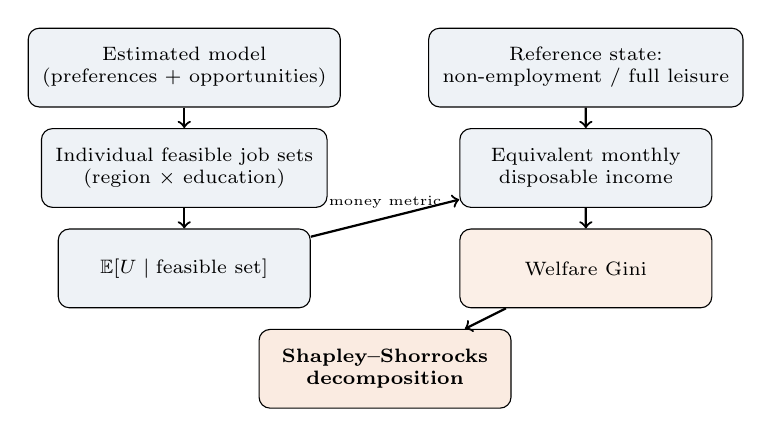
\begin{tikzpicture}[
  box/.style={draw,rounded corners,fill=cblue!8,minimum width=3.2cm,
    minimum height=1.0cm,font=\scriptsize,align=center,inner sep=5pt},
  scale=0.85]
  \node[box] (a) at (0,3) {Estimated model\\(preferences + opportunities)};
  \node[box] (b) at (0,1.5) {Individual feasible job sets\\(region $\times$ education)};
  \node[box] (c) at (0,0) {$\mathbb{E}[U \mid \text{feasible set}]$};
  \node[box] (d) at (6,3) {Reference state:\\non-employment / full leisure};
  \node[box] (e) at (6,1.5) {Equivalent monthly\\disposable income};
  \node[box,fill=corange!12] (f) at (6,0) {Welfare Gini};
  \node[box,fill=corange!15,font=\scriptsize\bfseries] (g) at (3,-1.5) {Shapley--Shorrocks\\decomposition};
  \draw[->,thick] (a) -- (b);
  \draw[->,thick] (b) -- (c);
  \draw[->,thick] (d) -- (e);
  \draw[->,thick] (c) -- (e) node[midway,above,font=\tiny] {money metric};
  \draw[->,thick] (e) -- (f);
  \draw[->,thick] (f) -- (g);
\end{tikzpicture}
\end{center}

\medskip
\scriptsize
\textcolor{cgrey}{Welfare $\equiv$ the monthly disposable income at the reference state that makes the individual indifferent to her estimated constrained-choice environment. Comparable across individuals while respecting heterogeneous opportunity sets.}
\end{frame}

% ---- APPENDIX 7: Full decomposition table ---------------------------
\begin{frame}{Appendix 7: Full Decomposition Table}

\begin{columns}[T]
\begin{column}{0.45\textwidth}
\centering
\footnotesize
\textbf{Counterfactual welfare Gini}\\[4pt]
\begin{tabular}{@{}l r r@{}}
\toprule
\textbf{Scenario} & \textbf{Gini} & \textbf{$\Delta$ vs baseline} \\
\midrule
Baseline            & 0.186 & --- \\
Opp.\ equalized     & 0.151 & $-$0.035 \\
Pref.\ equalized    & 0.140 & $-$0.046 \\
Both equalized      & 0.097 & $-$0.089 \\
\bottomrule
\end{tabular}
\end{column}
\begin{column}{0.50\textwidth}
\centering
\footnotesize
\textbf{Shapley--Shorrocks attribution}\\[4pt]
\begin{tabular}{@{}l r r r@{}}
\toprule
 & \textbf{Abs.} & \textbf{\% expl.} & \textbf{\% Gini} \\
\midrule
Opportunity     & 0.039 & 43.8\% & 21.0\% \\
Preference      & 0.050 & 56.2\% & 26.9\% \\
Residual/common & 0.097 & ---    & 52.2\% \\
\bottomrule
\end{tabular}
\end{column}
\end{columns}

\bigskip
\centering
\footnotesize
\textbf{Welfare distribution summary}\\[4pt]
\begin{tabular}{@{}cccc|cc@{}}
\toprule
Mean & Median & P10 & P90 & Inc.\ Gini & Welfare Gini \\
\midrule
\texteuro1,718 & \texteuro1,681 & \texteuro1,079 & \texteuro2,452 & 0.164 & 0.186 \\
\bottomrule
\end{tabular}
\end{frame}

% ---- APPENDIX 8: Responsibility-sensitivity table -------------------
\begin{frame}{Appendix 8: Responsibility-Sensitivity Table}

\centering
\footnotesize
\begin{tabular}{@{}l ccccc@{}}
\toprule
\textbf{Compensable} & \textbf{Opp.-eq.} & \textbf{Both-eq.} & \textbf{Shapley} & \textbf{Share of} & \textbf{Share of} \\
\textbf{definition}  & \textbf{Gini}      & \textbf{Gini}     & \textbf{opp.\ comp.} & \textbf{expl.\ red.} & \textbf{baseline} \\
\midrule
Region $\times$ ed.\ (baseline) & 0.151 & 0.097 & 0.039 & 43.8\% & 21.0\% \\
Education only                    & 0.158 & 0.105 & 0.031 & 38.9\% & 16.7\% \\
Region only                       & 0.164 & 0.110 & 0.026 & 34.2\% & 14.0\% \\
\bottomrule
\end{tabular}

\bigskip
\begin{itemize}\footnotesize
\item Tightening the responsibility stance reduces the compensable opportunity share, as expected
\item Even under the strictest stance, unequal opportunities still explain about \emphnum{14\%} of baseline welfare inequality
\item The contribution is the decomposition under \emph{explicit} responsibility assumptions, not one preferred criterion
\end{itemize}
\end{frame}

% ---- APPENDIX 9: Elasticity table and definition --------------------
\begin{frame}{Appendix 9: Elasticity Table and Definition}

\footnotesize
\textbf{Definition.}\; Uncompensated arc elasticities from a 1\% proportional increase in the gross wage attached to all working packages, holding the estimated opportunity mechanism (job-offer probabilities) fixed.

\bigskip
\centering
\begin{tabular}{@{}l ccc@{}}
\toprule
\textbf{Group} & \textbf{Extensive margin} & \textbf{Intensive margin} & \textbf{Total hours} \\
\midrule
Overall sample   & 0.21 & 0.11 & 0.32 \\
Low education    & 0.30 & 0.13 & 0.43 \\
Medium education & 0.22 & 0.11 & 0.33 \\
High education   & 0.14 & 0.09 & 0.23 \\
\bottomrule
\end{tabular}

\bigskip
\begin{itemize}\footnotesize
\item Most heterogeneity appears on the \textbf{extensive margin}
\item Lower-education women are more participation-responsive, consistent with weaker opportunity access
\item A 10\% wage increase would move employment from about 77.6\% to 79.2\% and mean hours from 34.9 to 35.3
\item This is a \textbf{behavioral-validation} object, not the paper's headline contribution
\end{itemize}
\end{frame}

\end{document}
